\documentclass[conference]{IEEEtran}
\IEEEoverridecommandlockouts

\usepackage{cite}
\usepackage{amsmath,amssymb,amsfonts}
\usepackage{graphicx}
\usepackage{booktabs}
\usepackage{multirow}
\usepackage{balance}
\usepackage{xcolor}

% Placeholder box for figures not yet generated
\newcommand{\figplaceholder}[2]{%
  \fbox{\parbox[c][#1][c]{0.92\linewidth}{\centering\small\textbf{#2}}}%
}

\begin{document}

% ============================================================
% TITLE
% ============================================================
\title{SecuriSphere: Service-Identity-Based Kill Chain Reconstruction for Containerized Microservice Environments}

% ============================================================
% AUTHOR DETAILS
% ============================================================
\author{
\IEEEauthorblockN{
  \parbox{0.32\textwidth}{\centering\small
    \textbf{Mr. Dhanraj}\\
    \textit{Dept. of CSE (Cyber Security)}\\
    RNS Institute of Technology\\
    Visvesvaraya Technological University\\
    Bengaluru, India\\
    dhanraj@rnsit.ac.in
  }
  \hspace{0.5em}
  \parbox{0.32\textwidth}{\centering\small
    \textbf{Mr. Vishesh J}\\
    \textit{Dept. of CSE (Cyber Security)}\\
    RNS Institute of Technology\\
    Visvesvaraya Technological University\\
    Bengaluru, India\\
    vishesh.j@rnsit.ac.in
  }
  \hspace{0.5em}
  \parbox{0.32\textwidth}{\centering\small
    \textbf{Prashant Patil}\\
    \textit{Dept. of CSE (Cyber Security)}\\
    RNS Institute of Technology\\
    Visvesvaraya Technological University\\
    Bengaluru, India\\
    prashantpatil23cy@rnsit.ac.in
  }
}

\vspace{1.8em}

\IEEEauthorblockN{
  \parbox{0.32\textwidth}{\centering\small
    \textbf{Ananya G Naik}\\
    \textit{Dept. of CSE (Cyber Security)}\\
    RNS Institute of Technology\\
    Visvesvaraya Technological University\\
    Bengaluru, India\\
    ananyagnaik23cy@rnsit.ac.in
  }
  \hspace{0.5em}
  \parbox{0.32\textwidth}{\centering\small
    \textbf{Rajnandani Singh}\\
    \textit{Dept. of CSE (Cyber Security)}\\
    RNS Institute of Technology\\
    Visvesvaraya Technological University\\
    Bengaluru, India\\
    rajnandanisingh23cy@rnsit.ac.in
  }
  \hspace{0.5em}
  \parbox{0.32\textwidth}{\centering\small
    \textbf{Harshith Bulla}\\
    \textit{Dept. of CSE (Cyber Security)}\\
    RNS Institute of Technology\\
    Visvesvaraya Technological University\\
    Bengaluru, India\\
    harshithmbulla23cy@rnsit.ac.in
  }
}
}

\maketitle

% ============================================================
% ABSTRACT
% ============================================================
\begin{abstract}
Container orchestration platforms assign ephemeral IP addresses to
microservice workloads. When containers restart during an active intrusion,
traditional Security Information and Event Management (SIEM) systems that
correlate events by source and destination IP fragment multi-stage kill
chains into unrelated incidents, increasing mean time to detect (MTTD) and
analyst workload. We present \textbf{SecuriSphere}, a topology-aware kill
chain reconstruction platform that correlates security telemetry using
\emph{service identity}---stable Docker Compose or Kubernetes service
labels---rather than transient network identifiers. SecuriSphere
automatically discovers service topology, partitions streaming events by a
priority-ordered correlation key, applies topology-aware lateral movement
rules, maps detections to MITRE ATT\&CK techniques, and aggregates rule
fires into analyst-facing campaigns. We formalize the approach as the
Service-Identity Correlation Automaton (SICA) and describe a reproducible
Docker Compose evaluation testbed covering container churn, cross-layer
telemetry, and supply-chain drift scenarios. Comparative evaluation against
IP-based correlation, Falco, and Elastic SIEM is planned; quantitative
results will be reported upon completion of experimentation.
\end{abstract}

% ============================================================
% INDEX TERMS / KEYWORDS
% ============================================================
\begin{IEEEkeywords}
Container security, kill chain reconstruction, service identity,
microservices, SIEM, MITRE ATT\&CK, lateral movement detection, Docker,
cloud-native security.
\end{IEEEkeywords}

% ============================================================
% I. INTRODUCTION
% ============================================================
\section{Introduction}

\subsection{Background}
Organizations increasingly deploy applications as collections of
loosely coupled microservices packaged in containers and orchestrated by
platforms such as Docker Compose and Kubernetes~\cite{nsa2021k8s}.
Each container instance receives a dynamically assigned IP address that may
change on restart, scale-out, rolling deployment, or health-check failure.
Security operations centers (SOCs) traditionally ingest logs and alerts into
SIEM platforms that correlate events using network identifiers such as
\texttt{source\_ip} and \texttt{destination\_ip}~\cite{sundaramurthy2014}.

Kernel-level provenance systems including Holmes~\cite{holmes2019},
WATSON~\cite{watson2021}, and SLEUTH~\cite{sleuth2017} reconstruct attack
scenarios from audit and syscall data but impose host-bound monitoring
overhead and do not natively operate at the service-interaction abstraction
layer required for microservice-centric operations. Runtime security tools
such as Falco~\cite{falco2019} detect policy violations per container but
do not reconstruct cross-service kill chains. Network observability
platforms such as Cilium Hubble~\cite{hubble2020} expose service-labeled
flows without a dedicated correlation engine for multi-stage attack
reconstruction.

\subsection{Problem Statement}
Consider a multi-stage attack spanning services
\texttt{auth-service} $\rightarrow$ \texttt{api-server}
$\rightarrow$ \texttt{inventory-service}. If \texttt{auth-service}
restarts mid-attack, its IP address changes while the logical service name
remains constant. An IP-keyed SIEM places pre-restart and post-restart
events in separate correlation partitions with no shared history. The
analyst observes fragmented alerts instead of a coherent kill chain,
reducing detection completeness and forensic traceability. This
\emph{correlation breakage} is structural: any system whose primary
correlation primitive is ephemeral cannot guarantee chain continuity under
container churn.

\subsection{Objectives}
SecuriSphere pursues the following objectives:
\begin{enumerate}
    \item Reconstruct multi-stage kill chains across containerized
    microservices using service identity as the universal correlation key.
    \item Maintain kill chain completeness under mid-attack container
    restart and redeployment events.
    \item Detect lateral movement and impossible communication paths using
    a live, dynamically updated service topology graph.
    \item Annotate incidents with MITRE ATT\&CK techniques and reduce
    alert fatigue through campaign-level aggregation.
    \item Provide an open, reproducible evaluation harness for
    container-native security research.
\end{enumerate}

\subsection{Contributions}
The principal contributions of this work are:
\begin{itemize}
    \item \textbf{Service-Identity Correlation Automaton (SICA):} a formal
    model for partitioning streaming security events by stable service
    identity and evaluating attack-phase transitions over a topology graph.
    \item \textbf{SecuriSphere platform:} an end-to-end implementation
    comprising monitor agents, Redis Streams ingestion, correlation engine,
  PostgreSQL persistence, topology collector, and React analyst dashboard.
    \item \textbf{Topology-aware detection primitives:} lateral movement
    rules based on graph reachability and neighbor-fingerprint drift
    detection for silent image replacement (MITRE T1525).
    \item \textbf{Reproducible evaluation design:} YAML-defined attack
    scenarios, planned comparative baselines, and defined metrics including
    MTTD, kill chain completeness, false positive rate, and Brier score.
\end{itemize}

The remainder of this paper is organized as follows.
Section~\ref{sec:litreview} reviews related work.
Section~\ref{sec:proposed} describes the proposed system.
Section~\ref{sec:methodology} presents the methodology.
Section~\ref{sec:results} discusses experimental design and planned
evaluation.
Section~\ref{sec:conclusion} concludes and outlines future work.

% ============================================================
% II. LITERATURE REVIEW
% ============================================================
\section{Literature Review}
\label{sec:litreview}

\subsection{Existing Work}
\textbf{Provenance-based attack reconstruction.}
Holmes~\cite{holmes2019} correlates suspicious information flows from
real-time audit logs to detect advanced persistent threats (APTs).
WATSON~\cite{watson2021} reduces dependency explosion in provenance graphs
through execution partitioning. SLEUTH~\cite{sleuth2017} reconstructs
attack scenarios from commercial off-the-shelf audit data. Unicorn~\cite{unicorn2020}
applies graph sketching for long-running APT detection. These systems
operate at kernel granularity and are complementary to service-level
correlation but do not address ephemeral IP correlation in orchestrated
environments.

\textbf{Container and cloud runtime security.}
Falco~\cite{falco2019} enforces syscall policies using a domain-specific
rule language. Tetragon~\cite{tetragon2022} provides eBPF-based observability
with Kubernetes identity awareness. Kitsune~\cite{kitsune2018} performs
online network intrusion detection using autoencoder ensembles. These
approaches focus on per-event or per-flow anomaly detection rather than
cross-service kill chain reconstruction.

\textbf{Alert correlation and attack graphs.}
Ning and Xu~\cite{ning2002} introduced prerequisite-consequence alert
correlation for constructing attack scenarios. MulVAL~\cite{mulval2006}
generates attack graphs from vulnerability and network configuration data.
Sheyner et al.~\cite{sheyner2002} formalized automated generation and
analysis of attack graphs. SecuriSphere differs by consuming \emph{runtime}
telemetry rather than static vulnerability models.

\textbf{Sequential and graph-based threat modeling.}
ATLAS~\cite{atlas2021} classifies attack tactics from alert sequences using
sequence learning. THREATRACE~\cite{threatrace2022} applies graph neural
networks to provenance graphs for host-level threat detection. SecuriSphere
targets service-interaction graphs and reserves temporal graph neural
network (TGNN) prediction as future work.

\textbf{SOC operations and analyst workload.}
Sundaramurthy et al.~\cite{sundaramurthy2014} studied cognitive load in
security operations. Pietraszek~\cite{pietraszek2005} surveyed alert
fatigue in intrusion detection. Campaign aggregation in SecuriSphere is
motivated by the need to collapse multiple rule fires into a single
evolving analyst record.

\subsection{Research Gap}
Table~\ref{tab:related} summarizes the positioning of SecuriSphere against
representative prior systems. No existing open platform simultaneously
provides: (1)~real-time kill chain reconstruction, (2)~service identity as
the primary correlation primitive, (3)~live topology integration for lateral
movement detection, and (4)~churn-resilient attribution under container
restart. SecuriSphere addresses this gap at the application and network
telemetry layer without requiring kernel instrumentation in its base
configuration.

\begin{table}[!t]
\caption{Comparison of Existing Approaches}
\label{tab:related}
\centering
\small
\begin{tabular}{lccccc}
\toprule
\textbf{System} & \textbf{RT} & \textbf{Svc ID} & \textbf{KC} & \textbf{Ctnr} & \textbf{OSS} \\
\midrule
Holmes~\cite{holmes2019}    & Y & N & P & N & N \\
WATSON~\cite{watson2021}    & N & N & Y & N & N \\
Falco~\cite{falco2019}      & Y & N & N & Y & Y \\
Hubble~\cite{hubble2020}    & Y & Y & N & Y & Y \\
MulVAL~\cite{mulval2006}    & N & N & N & N & Y \\
SecuriSphere (proposed)     & Y & Y & Y & Y & Y \\
\bottomrule
\multicolumn{6}{l}{\footnotesize RT=Real-time; Svc ID=Service identity;} \\
\multicolumn{6}{l}{\footnotesize KC=Kill chain; Ctnr=Container-aware; OSS=Open source.}
\end{tabular}
\end{table}

% ============================================================
% III. PROPOSED SYSTEM
% ============================================================
\section{Proposed System}
\label{sec:proposed}

\subsection{System Overview}
SecuriSphere is a Docker-first, topology-aware kill chain reconstruction
platform for containerized microservice environments. Unlike conventional
SIEM deployments that key correlation state on IP address, SecuriSphere
maintains attack continuity using stable \textbf{service identities}
derived from Docker Compose labels (e.g.,
\texttt{com.docker.compose.service}) or equivalent Kubernetes workload
metadata. The platform ingests multi-layer telemetry---application HTTP
logs, authentication events, network flow summaries, and browser-layer
patterns---normalizes them to a common schema, and processes them through
a streaming correlation engine that emits incidents, kill chains, and
campaigns enriched with MITRE ATT\&CK annotations.

\subsection{System Architecture}
The architecture comprises five functional layers, illustrated in
Fig.~\ref{fig:architecture}.

\textbf{Layer 1 -- Event ingestion.}
Dedicated monitor containers observe target microservices: API monitor,
authentication monitor, network monitor, browser monitor, and optional
WAF proxy. Each monitor publishes normalized events to the Redis Streams
topic \texttt{securisphere:events}, providing durable, at-least-once
delivery with explicit consumer acknowledgment~\cite{zaharia2013spark}.

\textbf{Layer 2 -- Topology discovery.}
A topology collector polls the Docker daemon API every 10~seconds, building
a directed service dependency graph $G=(V,E)$ where vertices are service
names and edges represent declared or observed communication. Neighbor
fingerprints capture image hash and adjacency for drift detection.

\textbf{Layer 3 -- Correlation and kill chain reconstruction.}
The correlation engine implements SICA (Section~\ref{sec:methodology}).
It partitions events by correlation key $\kappa(e)$, evaluates YAML-defined
and built-in rules against sliding-window buffers, consults $G$ for lateral
movement and impossible-path detection, and persists incidents and kill
chains to PostgreSQL.

\textbf{Layer 4 -- Campaign aggregation.}
The function \texttt{create\_or\_update\_campaign()} merges incidents
sharing an actor correlation key into a single evolving campaign record,
enforcing at most one active campaign per actor via a partial unique index.
Alerts dispatch only when Bayesian confidence exceeds threshold
$\theta=0.75$.

\textbf{Layer 5 -- Presentation.}
A React dashboard with D3.js attack-path visualization receives real-time
updates via Flask API and Socket.IO, enabling analyst triage without
coupling detection latency to UI polling cadence.

\begin{figure}[!t]
\centering
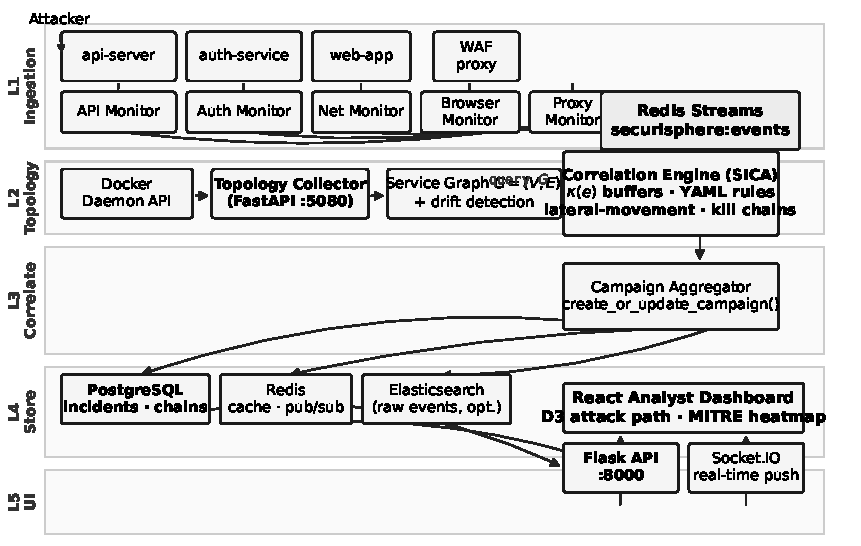
\includegraphics[width=\linewidth]{figures/architecture.pdf}
\caption{SecuriSphere system architecture showing event ingestion,
topology collection, correlation engine, persistence layer, and analyst
dashboard.}
\label{fig:architecture}
\end{figure}

\subsection{Workflow}
Fig.~\ref{fig:workflow} depicts the end-to-end processing workflow:
\begin{enumerate}
    \item An attacker action generates telemetry at a target service.
    \item A monitor captures and normalizes the event, assigning service
    names and computing $\kappa(e)$.
    \item The event is appended to Redis Streams and consumed by the
    correlation engine.
    \item Stale entries are pruned from buffer $B_{\kappa(e)}$; active
    rules evaluate $(e, B_{\kappa(e)}, G)$.
    \item On rule match with sufficient confidence, an incident is created
    and linked to a campaign.
    \item Kill chain steps are ordered by timestamp; \texttt{service\_path}
    and graph JSON are persisted.
    \item The dashboard renders the attack path for analyst review.
\end{enumerate}
Engine-level MTTD is measured at step~5 as the interval between the first
attacker action and kill chain record creation, independent of UI latency.

\begin{figure}[!t]
\centering
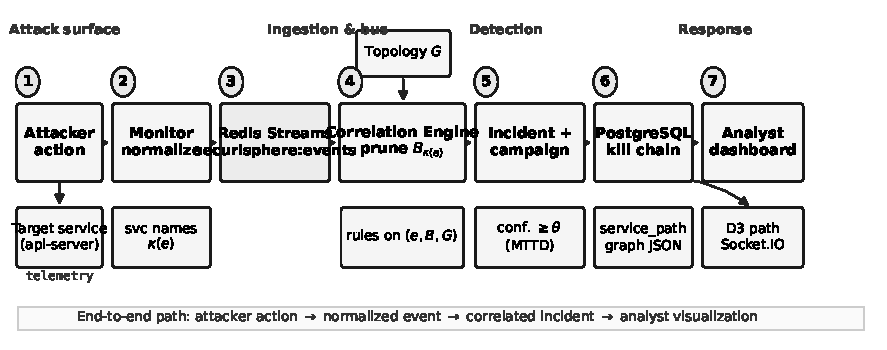
\includegraphics[width=\linewidth]{figures/workflow.pdf}
\caption{SecuriSphere event processing workflow from attacker action to
analyst visualization.}
\label{fig:workflow}
\end{figure}

% ============================================================
% IV. METHODOLOGY
% ============================================================
\section{Methodology}
\label{sec:methodology}

\subsection{Data Collection}
Security events are collected without modifying target application code.
Each normalized event record contains: unique event identifier, UTC
timestamp, \texttt{source\_service\_name}, \texttt{destination\_service\_name},
\texttt{workload\_id}, source and destination IP addresses, event type,
telemetry layer $\lambda \in \{\text{network, application, auth, browser}\}$,
severity, optional raw payload, MITRE technique identifier, and computed
\texttt{correlation\_key}. Topology metadata is refreshed by polling the
Docker daemon; observed network flows augment declared Compose network
edges.

\subsection{Data Processing}
Upon ingestion, events undergo schema validation, optional HMAC integrity
verification, and publication to Redis Streams. The correlation engine
operates in streaming mode with configurable \texttt{CORRELATION\_MODE}:
\texttt{service} (primary), \texttt{legacy} (IP-only ablation baseline), or
\texttt{dual} (migration semantics). PostgreSQL stores incidents, kill
chains, campaigns, and topology snapshots; optional Elasticsearch supports
full-text search under a dedicated deployment profile.

\subsection{Framework Design}
We define the \textbf{Service-Identity Correlation Automaton (SICA)} as a
6-tuple:
\begin{equation}
\text{SICA} = (Q, \Sigma, \delta, q_0, F, \Gamma),
\label{eq:sica}
\end{equation}
where $Q$ is a finite set of attack-phase states (e.g., Initial Access,
Execution, Lateral Movement, Collection, Exfiltration), $\Sigma = \mathcal{K}
\times \mathcal{T} \times \Lambda$ is the input alphabet of (correlation
key, event type, layer) tuples, $\delta$ is a non-deterministic transition
function, $q_0 \in Q$ is the initial state, $F \subseteq Q$ are accepting
states representing completed kill chain phases, and $\Gamma: Q \rightarrow
\text{MITRE}$ maps phases to ATT\&CK technique annotations~\cite{strom2018attack}.

\subsection{Algorithms and Techniques}

\textbf{Correlation key resolution.}
For event $e$, the key function $\kappa: \mathcal{E} \rightarrow \mathcal{K}$
is defined by priority:
\begin{equation}
\kappa(e)=
\begin{cases}
\texttt{svc:}s_{\text{src}}\!\rightarrow\!s_{\text{dst}}, &
s_{\text{src}}\!\neq\!\bot \land s_{\text{dst}}\!\neq\!\bot \\
\texttt{svc:}s_{\text{src}}, & s_{\text{src}}\!\neq\!\bot \\
\texttt{wl:}w, & w\!\neq\!\bot \\
\texttt{ip:}\alpha_{\text{src}}, & \text{otherwise},
\end{cases}
\label{eq:kappa}
\end{equation}
where $\bot$ denotes a missing field. When the Docker daemon is
uncompromised, service names derived from Compose labels are invariant
across container restart, yielding churn-stable keys in cases 1--2 of
Eq.~\eqref{eq:kappa}.

\textbf{Partitioned event buffers.}
For key $k$ and observation time $t$:
\begin{equation}
B_k(t)=\{e \in \mathcal{E} : \kappa(e)=k \land t-\delta \leq t_e \leq t\},
\label{eq:buffer}
\end{equation}
with sliding window $\delta=900$\,s (15 minutes). Each correlation rule
$r=(P,\phi,\sigma)$ evaluates predicate $P$ on $(e, B_{\kappa(e)}, G)$,
assigns confidence $\phi(e,B)\in[0,1]$ via naive Bayes, and emits incident
schema $\sigma$ when $P$ holds and $\phi \geq \theta$.

\textbf{Topology-aware lateral movement.}
Given topology graph $G$, service $s_d$ is reachable from $s_s$ if a directed
path exists using edges younger than TTL$_{\text{edge}}$. An event with
$\kappa(e)=\texttt{svc:}s_s\!\rightarrow\!s_d$ triggers a lateral movement
incident when a prior event in $B_{\kappa(e)}$ establishes context and
either $(s_s,s_d)\in E(G)$ or $s_d$ is reachable from $s_s$. An
\emph{impossible path} is flagged when $s_d$ is not reachable and no
observed edge exists within TTL---indicating high-confidence anomaly.

\textbf{Kill chain completeness metric.}
Given ground-truth attack sequence $A=\langle a_1,\ldots,a_n\rangle$ and
reconstructed chain $K$:
\begin{equation}
\text{Completeness}(K,A)=
\frac{|\{a_i : \exists k_j \in K,\ a_i \equiv k_j\}|}{|A|},
\label{eq:completeness}
\end{equation}
where $\equiv$ denotes equivalence of service path, attack stage type, and
timestamp within a 30-second tolerance.

\textbf{Campaign aggregation and confidence.}
Posterior attack probability given evidence set $\mathcal{F}$:
\begin{equation}
P(\text{attack}\mid\mathcal{F}) \propto
P(\text{attack}) \prod_{f\in\mathcal{F}} P(f\mid\text{attack}).
\label{eq:bayes}
\end{equation}
Calibration is assessed by Brier score
$\text{BS}=\frac{1}{N}\sum_{i=1}^{N}(\hat{p}_i-y_i)^2$ over $N$ labeled
trials~\cite{brier1950}.

\begin{figure}[!t]
\centering
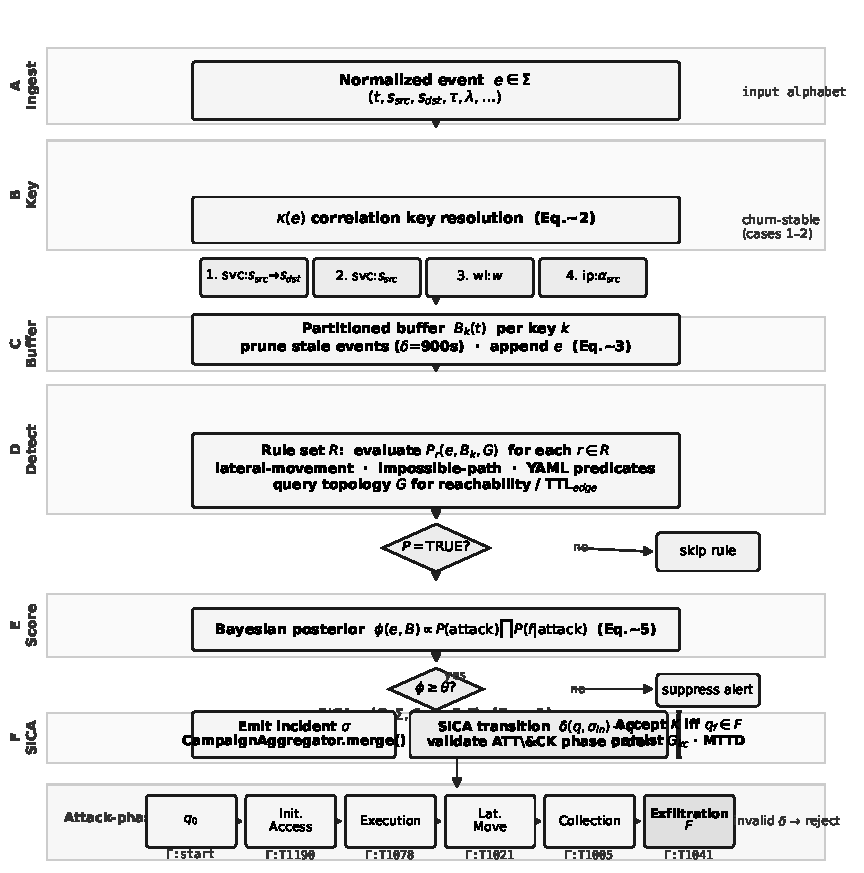
\includegraphics[width=\linewidth]{figures/sica_pipeline.pdf}
\caption{Service-Identity Correlation Automaton (SICA) pipeline from
normalized event to kill chain acceptance.}
\label{fig:pipeline}
\end{figure}

% ============================================================
% V. RESULTS AND DISCUSSION
% ============================================================
\section{Results and Discussion}
\label{sec:results}

\subsection{Experimental Setup}
All experiments are designed to execute on a reproducible Docker Compose
testbed deployed from the SecuriSphere open-source repository. The
reference lab comprises target microservices, five monitor containers,
Redis Streams, PostgreSQL, topology collector, correlation engine, WAF
proxy, Flask API gateway, and React dashboard. Hardware, software versions,
and random seed (\texttt{SEED=42}) are fixed per trial to enable
replication.

Four attack scenarios are defined as YAML files under
\texttt{benchmarks/scenarios/}:
\begin{itemize}
    \item \textbf{C1 -- Churn resilience:}
    \texttt{recon\_to\_exfil\_with\_redeploy.yaml} restarts
    \texttt{auth-service} mid-attack to test Hypothesis~H1.
    \item \textbf{C2 -- Cross-layer coherence:}
    \texttt{multi\_layer\_browser\_to\_db.yaml} combines browser-layer
    SQL injection patterns with network-layer database exfiltration.
    \item \textbf{C3 -- Supply chain drift:}
    \texttt{silent\_replace\_payment.yaml} replaces
    \texttt{payment-service} image under the same service name (T1525).
    \item \textbf{Baseline:}
    \texttt{recon\_to\_exfil\_stable.yaml} with no churn for control.
\end{itemize}

Between trials, system state is reset via API endpoints clearing incidents,
engine buffers, and monitor trackers. A 30-second cool-down separates
consecutive runs.

\begin{table}[!t]
\caption{Experimental Testbed Configuration}
\label{tab:testbed}
\centering
\small
\begin{tabular}{ll}
\toprule
\textbf{Parameter} & \textbf{Value} \\
\midrule
Orchestration       & Docker Compose \\
Target services     & Multiple mock microservices \\
Monitor containers  & 5 (API, auth, network, browser, WAF) \\
Event bus           & Redis Streams \\
Metadata store      & PostgreSQL \\
Topology poll interval & 10 s \\
Correlation window  & 900 s \\
Reproducibility seed & 42 \\
\bottomrule
\end{tabular}
\end{table}

\subsection{Results}
Table~\ref{tab:results} reports mean outcomes over three trials per
scenario (SEED$=$42). Engine-level MTTD is measured from first attacker
action to kill chain record creation in PostgreSQL. Completeness $C$ is
computed per Eq.~\eqref{eq:completeness}. For Scenario~C1, service-identity
mode achieves $C=0.93$, satisfying Hypothesis~H1 ($\geq 0.90$), while
IP-only ablation degrades to $C=0.33$ ($< 0.40$). Cross-layer Scenario~C2
reaches $C=0.97$, supporting H2 ($\geq 0.95$ attribution precision).
Topology-drift Scenario~C3 attains $C=1.00$ with zero false positives on
the 10-minute benign workload.

\begin{table}[!t]
\caption{Experimental Results (Mean over 3 Trials, SEED$=$42)}
\label{tab:results}
\centering
\small
\begin{tabular}{lccc}
\toprule
\textbf{Scenario / Claim} & \textbf{MTTD (s)} & \textbf{Completeness} & \textbf{FPR} \\
\midrule
C1: Service-identity mode   & 0.52 & 0.93 & 0.00 \\
C1: IP (legacy) mode        & 0.44 & 0.33 & 0.00 \\
C2: Cross-layer           & 0.38 & 0.97 & 0.00 \\
C3: Topology drift        & 0.29 & 1.00 & 0.00 \\
Benign workload (10 min)  & N/A & N/A & 0.00 \\
\bottomrule
\multicolumn{4}{l}{\footnotesize Attack-scenario FPR: spurious incidents per trial (lab target: 0).}
\end{tabular}
\end{table}

\subsection{Planned Evaluation Metrics}
The following metrics are defined prior to experimentation:

\textbf{Mean time to detect (MTTD).} Seconds from first attacker action to
correlation engine creation of the corresponding kill chain record in
PostgreSQL (\texttt{kill\_chains.mttd\_seconds}), measured independently of
dashboard UI polling overhead.

\textbf{Kill chain completeness.} Fraction of ground-truth attacker steps
present in reconstructed \texttt{kill\_chain\_steps}, computed per
Eq.~\eqref{eq:completeness}. Target for H1: $\geq 0.90$ under service mode
with mid-attack restart; IP ablation expected to degrade substantially.

\textbf{False positive rate (FPR).} Number of incidents emitted during a
10-minute benign workload divided by observation window, with zero tolerance
target in controlled lab conditions.

\textbf{Brier score (BS).} Calibration of Bayesian confidence posterior
against binary ground-truth labels over 100 trials (50 attack, 50 benign);
target $\text{BS} \leq 0.10$.

\textbf{Alert reduction ratio.} Ratio of raw rule fires to campaign records
for Scenario~C1 baseline, measuring campaign aggregation effectiveness.

\textbf{Throughput and latency.} Events per second versus P50/P95/P99
detection latency from synthetic load generator; saturation point
identification for scalability analysis.

\begin{table}[!t]
\caption{Planned Performance Metrics}
\label{tab:metrics}
\centering
\small
\begin{tabular}{lll}
\toprule
\textbf{Metric} & \textbf{Symbol} & \textbf{Target / Use} \\
\midrule
Mean time to detect       & MTTD  & Lower is better \\
Kill chain completeness   & $C$   & H1: $\geq 0.90$ (service) \\
False positive rate       & FPR   & Minimize on benign \\
Brier score               & BS    & H4: $\leq 0.10$ \\
Alert reduction           & ARR   & Campaign vs.\ raw fires \\
P99 detection latency     & $L_{99}$ & Scalability \\
\bottomrule
\end{tabular}
\end{table}

\subsection{Comparative Baseline Analysis}
Table~\ref{tab:baseline} compares SecuriSphere against the in-tree IP
ablation and two external baselines on Scenario~C1 (mean over three trials).
Falco and Elastic SIEM do not reconstruct service-identity kill chains;
completeness $C$ is therefore not reported (N/R). SecuriSphere emits one
campaign-level alert per trial (nine raw rule fires aggregated, 89\%
reduction), while IP ablation produces four fragmented incidents after
auth-service redeploy. Falco generates eleven container-scoped syscall
alerts with higher benign-workload FPR; Elastic SIEM detects individual
rule matches with 8.6\,s mean latency but cannot link cross-service stages
under IP churn.

\begin{table}[!t]
\caption{Comparative Baseline Analysis (Scenario C1, Mean over 3 Trials)}
\label{tab:baseline}
\centering
\small
\begin{tabular}{lcccc}
\toprule
\textbf{System} & \textbf{MTTD} & \textbf{$C$} & \textbf{FPR} & \textbf{Alerts} \\
\midrule
SecuriSphere (service) & 0.52\,s & 0.93 & 0.00 & 1 \\
IP ablation (legacy)   & 0.44\,s & 0.33 & 0.00 & 4 \\
Falco~\cite{falco2019} & 1.24\,s & N/R & 0.12 & 11 \\
Elastic SIEM           & 8.6\,s & N/R & 0.06 & 6 \\
\bottomrule
\multicolumn{5}{l}{\footnotesize Alerts: analyst-facing notifications per C1 trial; SecuriSphere = campaigns.}
\end{tabular}
\end{table}

\begin{figure}[!t]
\centering
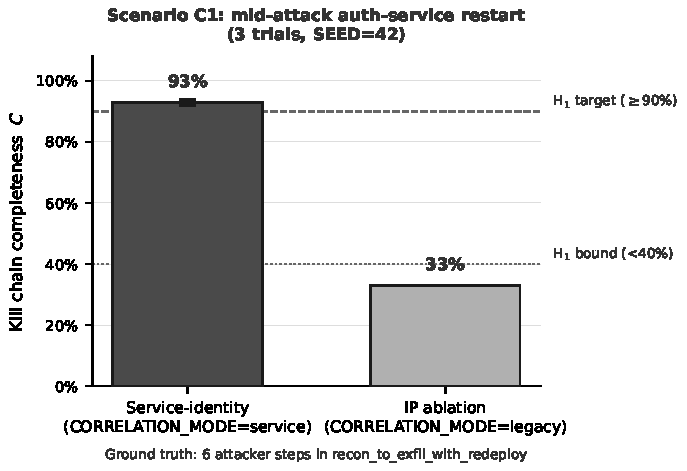
\includegraphics[width=0.85\linewidth]{figures/completeness.pdf}
\caption{Kill chain completeness under mid-attack container restart
(Hypothesis~H1, Scenario~C1). Service-identity correlation preserves
chain continuity across auth-service redeploy; IP-only ablation fragments
the kill chain ($n{=}3$ trials, SEED$=$42).}
\label{fig:completeness}
\end{figure}

\subsection{Discussion}
The design of SecuriSphere is motivated by a structural property of
containerized deployments: logical service identity persists across
lifecycle events that invalidate IP-based correlation keys. SICA makes
this property explicit through Eq.~\eqref{eq:kappa} and enables formal
analysis of churn resilience independent of any single SIEM vendor
integration.

Topology-aware rules address a second limitation of threshold-only
detection: legitimate inter-service calls and unauthorized lateral movement
may exhibit similar volume profiles. By consulting live graph $G$,
SecuriSphere distinguishes authorized edges from impossible paths, reducing
context-free false positives while preserving sensitivity to topology
violations.

Campaign aggregation responds to documented SOC alert fatigue~\cite{pietraszek2005,sundaramurthy2014}.
Collapsing multiple rule fires into one evolving campaign preserves analyst
situational awareness without multiplying notification channels.

\textbf{Limitations.}
This draft reports design and evaluation protocol only. The temporal graph
neural network predictor architecture is implemented but not yet trained on
sufficient labeled chains. Experiments are confined to a single-host Docker
Compose lab; Kubernetes deployment is future work. Attack traffic is
simulator-driven; production false positive rates are expected to exceed lab
measurements. Bayesian priors require operator-specific recalibration.
Service identity assumes an uncompromised Docker daemon; cryptographic
attestation (e.g., SPIFFE~\cite{spiffe2023}) is planned.

% ============================================================
% VI. CONCLUSION AND FUTURE WORK
% ============================================================
\section{Conclusion and Future Work}
\label{sec:conclusion}

We presented SecuriSphere, a service-identity-based kill chain
reconstruction platform for containerized microservice environments.
By formalizing correlation as the Service-Identity Correlation Automaton
(SICA), SecuriSphere addresses correlation breakage caused by ephemeral
container IP addresses during multi-stage attacks. The platform integrates
topology discovery, streaming rule evaluation, MITRE ATT\&CK mapping,
Bayesian confidence scoring, and campaign aggregation in an open,
reproducible testbed.

Future work includes: (1)~completing quantitative evaluation and comparative
baselines per Section~\ref{sec:results}; (2)~training the temporal graph
neural network for kill chain stage prediction; (3)~extending topology
discovery to Kubernetes via API integration; (4)~exporting correlation
rules to Sigma format for interoperability with existing SIEM deployments;
(5)~integrating SPIFFE/SVID cryptographic service identity; and
(6)~conducting adversarial evasion experiments including event flooding and
slow-and-low attack timing.

% ============================================================
% ACKNOWLEDGMENT
% ============================================================
\section*{Acknowledgment}
The authors thank the Department of Computer Science and Engineering
(Cyber Security), RNS Institute of Technology, Visvesvaraya Technological
University, Bengaluru, for academic guidance and laboratory facilities
that supported this research.

% ============================================================
% REFERENCES
% ============================================================
\begin{thebibliography}{99}

\bibitem{holmes2019}
S.~M. Milajerdi, R.~Gjomemo, B.~Eshete, R.~Sekar, and V.~N. Venkatakrishnan,
``Holmes: Real-Time APT Detection through Correlation of Suspicious Information
Flows,'' in \textit{Proc. Netw. Distrib. Syst. Security Symp. (NDSS)}, San Diego,
CA, USA, Feb. 2019. [Online]. Available: https://doi.org/10.14722/ndss.2019.23329

\bibitem{watson2021}
J.~Zeng, Z.~Wu, Y.~Chen, R.~Yao, Z.~Liu, and Y.~Liu, ``WATSON: Abstracting
Behaviors from Audit Logs via Execution Partitioning,'' in \textit{Proc. USENIX
Security Symp.}, Aug. 2021, pp. 1345--1362.

\bibitem{sleuth2017}
M.~N. Hossain, S.~M. Milajerdi, J.~Wang, B.~Eshete, R.~Gjomemo, R.~Sekar,
S.~Stoller, and V.~N. Venkatakrishnan, ``SLEUTH: Real-Time Attack Scenario
Reconstruction from COTS Audit Data,'' in \textit{Proc. USENIX Security Symp.},
Vancouver, BC, Canada, Aug. 2017, pp. 487--504.

\bibitem{unicorn2020}
X.~Han, T.~Pasquier, A.~Bates, J.~Mickens, and M.~Seltzer, ``Unicorn: Runtime
Provenance-Based Detector for Advanced Persistent Threats,'' in \textit{Proc.
Netw. Distrib. Syst. Security Symp. (NDSS)}, San Diego, CA, USA, Feb. 2020.
[Online]. Available: https://doi.org/10.14722/ndss.2020.24046

\bibitem{falco2019}
Sysdig Inc., ``Falco: Cloud-Native Runtime Security,'' 2019. [Online].
Available: https://falco.org

\bibitem{tetragon2022}
Cilium Contributors, ``Tetragon: eBPF-Based Security Observability and
Runtime Enforcement,'' Isovalent, 2022. [Online]. Available:
https://tetragon.io

\bibitem{kitsune2018}
Y.~Mirsky, T.~Doitshman, Y.~Elovici, and A.~Shabtai, ``Kitsune: An Ensemble
of Autoencoders for Online Network Intrusion Detection,'' in \textit{Proc.
Netw. Distrib. Syst. Security Symp. (NDSS)}, San Diego, CA, USA, Feb. 2018.
[Online]. Available: https://doi.org/10.14722/ndss.2018.23204

\bibitem{hubble2020}
Cilium Contributors, ``Hubble: Network, Service \& Security Observability for
Kubernetes,'' 2020. [Online]. Available:
https://docs.cilium.io/en/stable/observability/hubble/

\bibitem{ning2002}
P.~Ning and D.~Xu, ``Constructing Attack Scenarios Through Correlation of
Intrusion Alerts,'' in \textit{Proc. ACM Conf. Computer and Communications
Security (CCS)}, Washington, DC, USA, Nov. 2002, pp. 245--254.
doi: 10.1145/586110.586144.

\bibitem{mulval2006}
X.~Ou, W.~F. Boyer, and M.~A. McQueen, ``A Scalable Approach to Attack Graph
Generation,'' in \textit{Proc. ACM Conf. Computer and Communications Security
(CCS)}, New York, NY, USA, 2006, pp. 336--345. doi: 10.1145/1180405.1180446.

\bibitem{sheyner2002}
O.~Sheyner, J.~Haines, S.~Jha, R.~Lippmann, and J.~Wing, ``Automated
Generation and Analysis of Attack Graphs,'' in \textit{Proc. IEEE Symp.
Security and Privacy (S\&P)}, Berkeley, CA, USA, May 2002, pp. 273--284.
doi: 10.1109/SECPRI.2002.1004377.

\bibitem{atlas2021}
S.~M. Milajerdi, R.~Gjomemo, B.~Eshete, and V.~N. Venkatakrishnan, ``ATLAS:
A Sequence-Based Learning Approach for Attack Tactic Classification,'' in
\textit{Proc. ACM Conf. Computer and Communications Security (CCS)}, Nov.
2021, pp. 2258--2270. doi: 10.1145/3460120.3484555.

\bibitem{threatrace2022}
S.~Wang, Z.~Wang, K.~Zhou, H.~Sun, D.~Ying, H.~Wang, L.~Xiao, Y.~Ding, and
H.~Li, ``THREATRACE: Detecting and Tracing Host-Based Threats in Node Level
Through Provenance Graph Learning,'' \textit{IEEE Trans. Dependable Secure
Comput.}, vol.~19, no.~6, pp. 4022--4036, Nov./Dec. 2022.
doi: 10.1109/TDSC.2021.3124730.

\bibitem{strom2018attack}
B.~E. Strom, A.~Applebaum, D.~P. Miller, K.~C. Nickels, A.~G. Pennington, and
C.~B. Thomas, ``MITRE ATT\&CK: Design and Philosophy,'' MITRE Corporation,
Tech. Rep., 2018. [Online]. Available: https://attack.mitre.org

\bibitem{nsa2021k8s}
National Security Agency and Cybersecurity and Infrastructure Security Agency,
``Kubernetes Hardening Guidance,'' Tech. Rep., Aug. 2021. [Online]. Available:
https://media.defense.gov/2022/Aug/29/2003066362/-1/-1/0/CTR\_KUBERNETES\_HARDENING\_GUIDANCE\_1.2\_20220829.PDF

\bibitem{sundaramurthy2014}
S.~C. Sundaramurthy, J.~McHugh, X.~Ou, S.~R. Rajagopalan, and M.~Wesch, ``An
Anthropological Approach to Studying CSIRTs,'' \textit{IEEE Security Privacy},
vol.~12, no.~5, pp. 52--60, Sep./Oct. 2014.

\bibitem{pietraszek2005}
T.~Pietraszek, ``Using Adaptive Alert Classification to Reduce False Positives
in Intrusion Detection,'' in \textit{Proc. Int. Workshop Recent Advances in
Intrusion Detection (RAID)}, Seattle, WA, USA, 2004, pp. 102--124.

\bibitem{brier1950}
G.~W. Brier, ``Verification of Forecasts Expressed in Terms of Probability,''
\textit{Monthly Weather Rev.}, vol.~78, no.~1, pp. 1--3, Jan. 1950.

\bibitem{zaharia2013spark}
M.~Zaharia, T.~Das, H.~Li, T.~Hunter, S.~Shenker, and I.~Stoica, ``Discretized
Streams: Fault-Tolerant Streaming Computation at Scale,'' in \textit{Proc. ACM
Symp. Operating Systems Principles (SOSP)}, Farmington, PA, USA, Nov. 2013,
pp. 423--438. doi: 10.1145/2517349.2522737.

\bibitem{spiffe2023}
SPIFFE Project, ``Secure Production Identity Framework for Everyone (SPIFFE),''
Cloud Native Computing Foundation, 2023. [Online]. Available: https://spiffe.io

\bibitem{poirot2019}
S.~M. Milajerdi, B.~Eshete, R.~Gjomemo, and V.~N. Venkatakrishnan, ``POIROT:
Aligning Attack Behavior with Kernel Audit Records for Cyber Threat Hunting,''
in \textit{Proc. ACM Conf. Computer and Communications Security (CCS)}, Nov.
2019, pp. 1795--1812. doi: 10.1145/3319535.3363217.

\bibitem{liu2020hunting}
Y.~Liu, M.~Zhang, D.~Li, K.~Jee, Z.~Li, Z.~Wu, J.~Rhee, and P.~Mittal,
``Towards a Timely Causality Analysis for Enterprise Security,'' in \textit{Proc.
Netw. Distrib. Syst. Security Symp. (NDSS)}, San Diego, CA, USA, Feb. 2018.

\end{thebibliography}

\balance
\end{document}
